\subsubsection{Problems and Solutions}
3D printing is typically an iterative process, where the design is printed, tested, and then modified based on the results.
This further reinforces the need for a modular and parametric design, as it allows for easy modification of each component.
After a few iterations with errors due to tolerances and slightly incorrect measurements, (not relevant to the technical content of this report)
a design was produced that physically fit together and mounted the components as intended, however when combined with the software
and electronics, a few problems were encountered that were overcome by making some design decisions that were discussed with the project's supervisor, Dr. Stott. \\

\begin{figure*}
    \begin{minipage}[t]{0.49\textwidth}
        \centering
        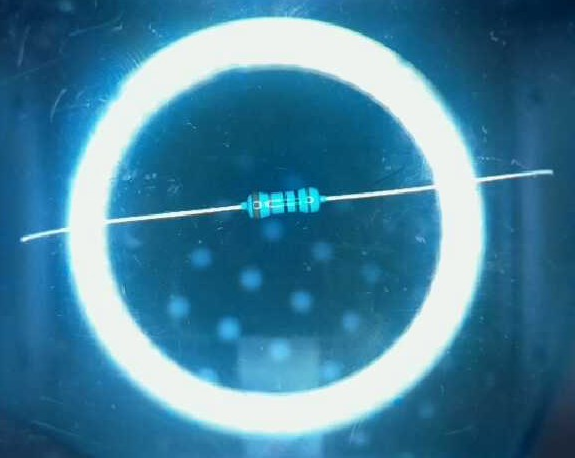
\includegraphics[width=\textwidth,height=7cm, keepaspectratio]{imgs/design/ringlight.jpg}
        \caption{Glare from LED Ring}
        \label{fig:glare}
    \end{minipage}
    \hfill
    \begin{minipage}[t]{0.49\textwidth}
        \centering
        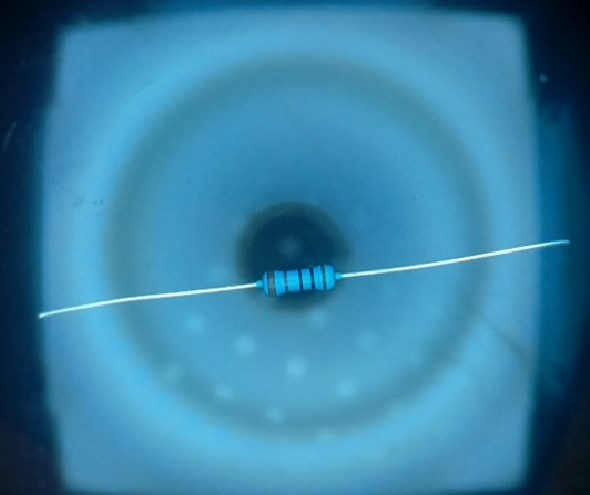
\includegraphics[width=\textwidth,height=7cm, keepaspectratio]{imgs/design/diffusedlight.jpg}
        \caption{Diffused Light}
        \label{fig:diffusedlight}
    \end{minipage}
\end{figure*}

\noindent
\textbf{Mechanical Design Problems} \\
The first design problem was the initial design of the LCD mount. As mentioned in Section \ref{sec:lcdhousing},
the LCD housing is split into two parts; the LCD cover, where the LCD slides into, and a base plate, which mounts to the camera housing.
The initial design of the LCD cover was only mounted to the base plate using two M3 screws at the base as shown in Figure \ref{fig:unbracedscreen}, which made it unstable and prone to wobbling.
Over time, this would put stress on the plastic, causing it to break. To solve this, a third mounting point was added to the LCD cover in the form of a 
brace that reaches halfway up the LCD cover, as shown in Figure \ref{fig:bracedscreen}, increasing the stability of the LCD, and preventing it from wobbling.

The second design problem was the design of the camera housing. As mentioned in Section \ref{sec:camerahousing}, the camera housing contains the camera and the LED strip.
The camera itself is not a macro lens, but rather a standard lens with an adjustable focus. The workaround is to set the focus as close as possible, and then determine the optimal
distance between the camera and the object to be imaged. This is done by placing an object on the acrylic plate. Initially, the height of the camera housing was too short as shown in Figure \ref{fig:shortcamera}, resulting in a 
blurry image, which was remedied by simply changing the parametric parameters that define the height of the camera housing, as shown in Figure \ref{fig:tallcamera}. 

The above design problems were solved by simply modifying the design, however, the third design problem was more complex. As mentioned in Section \ref{sec:camerahousing}, the approach 
to imaging components is to place them on the acrylic plate, and then image them using the camera. However, when doing so, the light from the LED Ring would reflect off the acrylic plate as shown by Figure \ref{fig:glare},
resulting in an incredible glare that would obscure the image of the component. There was an attempt to 3D print a light diffuser to reduce the glare Figure \ref{fig:diffusedlight}, however, this was not effective and instead
caused the entire image to be affected by the reflection of the LED Ring. This was a major design problem as, in the non-diffused image, any components in the glare of the ring were obscured, and in the diffused image,
the entire image had incorrect colours and was partially obscured. To solve this, three solutions were considered:
\begin{mylist}
  \item \textbf{Polarising Filter} \\
  Polarising filters can be used to reduce glare by filtering out light that is polarised in a certain direction.
  \item \textbf{Different Light Source} \\
  The LED Ring was chosen as it provides a uniform light source as it would surround the camera, however, it is possible to use a different light source that does not cause glare, for example,
  an LED strip that is mounted above the camera near the acrylic plate.
  \item \textbf{Down-facing Camera} \\
  Instead of imaging the components from below, the camera can be mounted such that it is facing down, and images the components from above, as explored in Section \ref{sec:background} (Background).
  The issue is that the light of the LED Ring bounces off the bottom layer of the acrylic plate, so any components on top are obscured.
\end{mylist}
  
\begin{figure*}[t]
  \begin{minipage}[t]{0.24\textwidth}
    \centering
    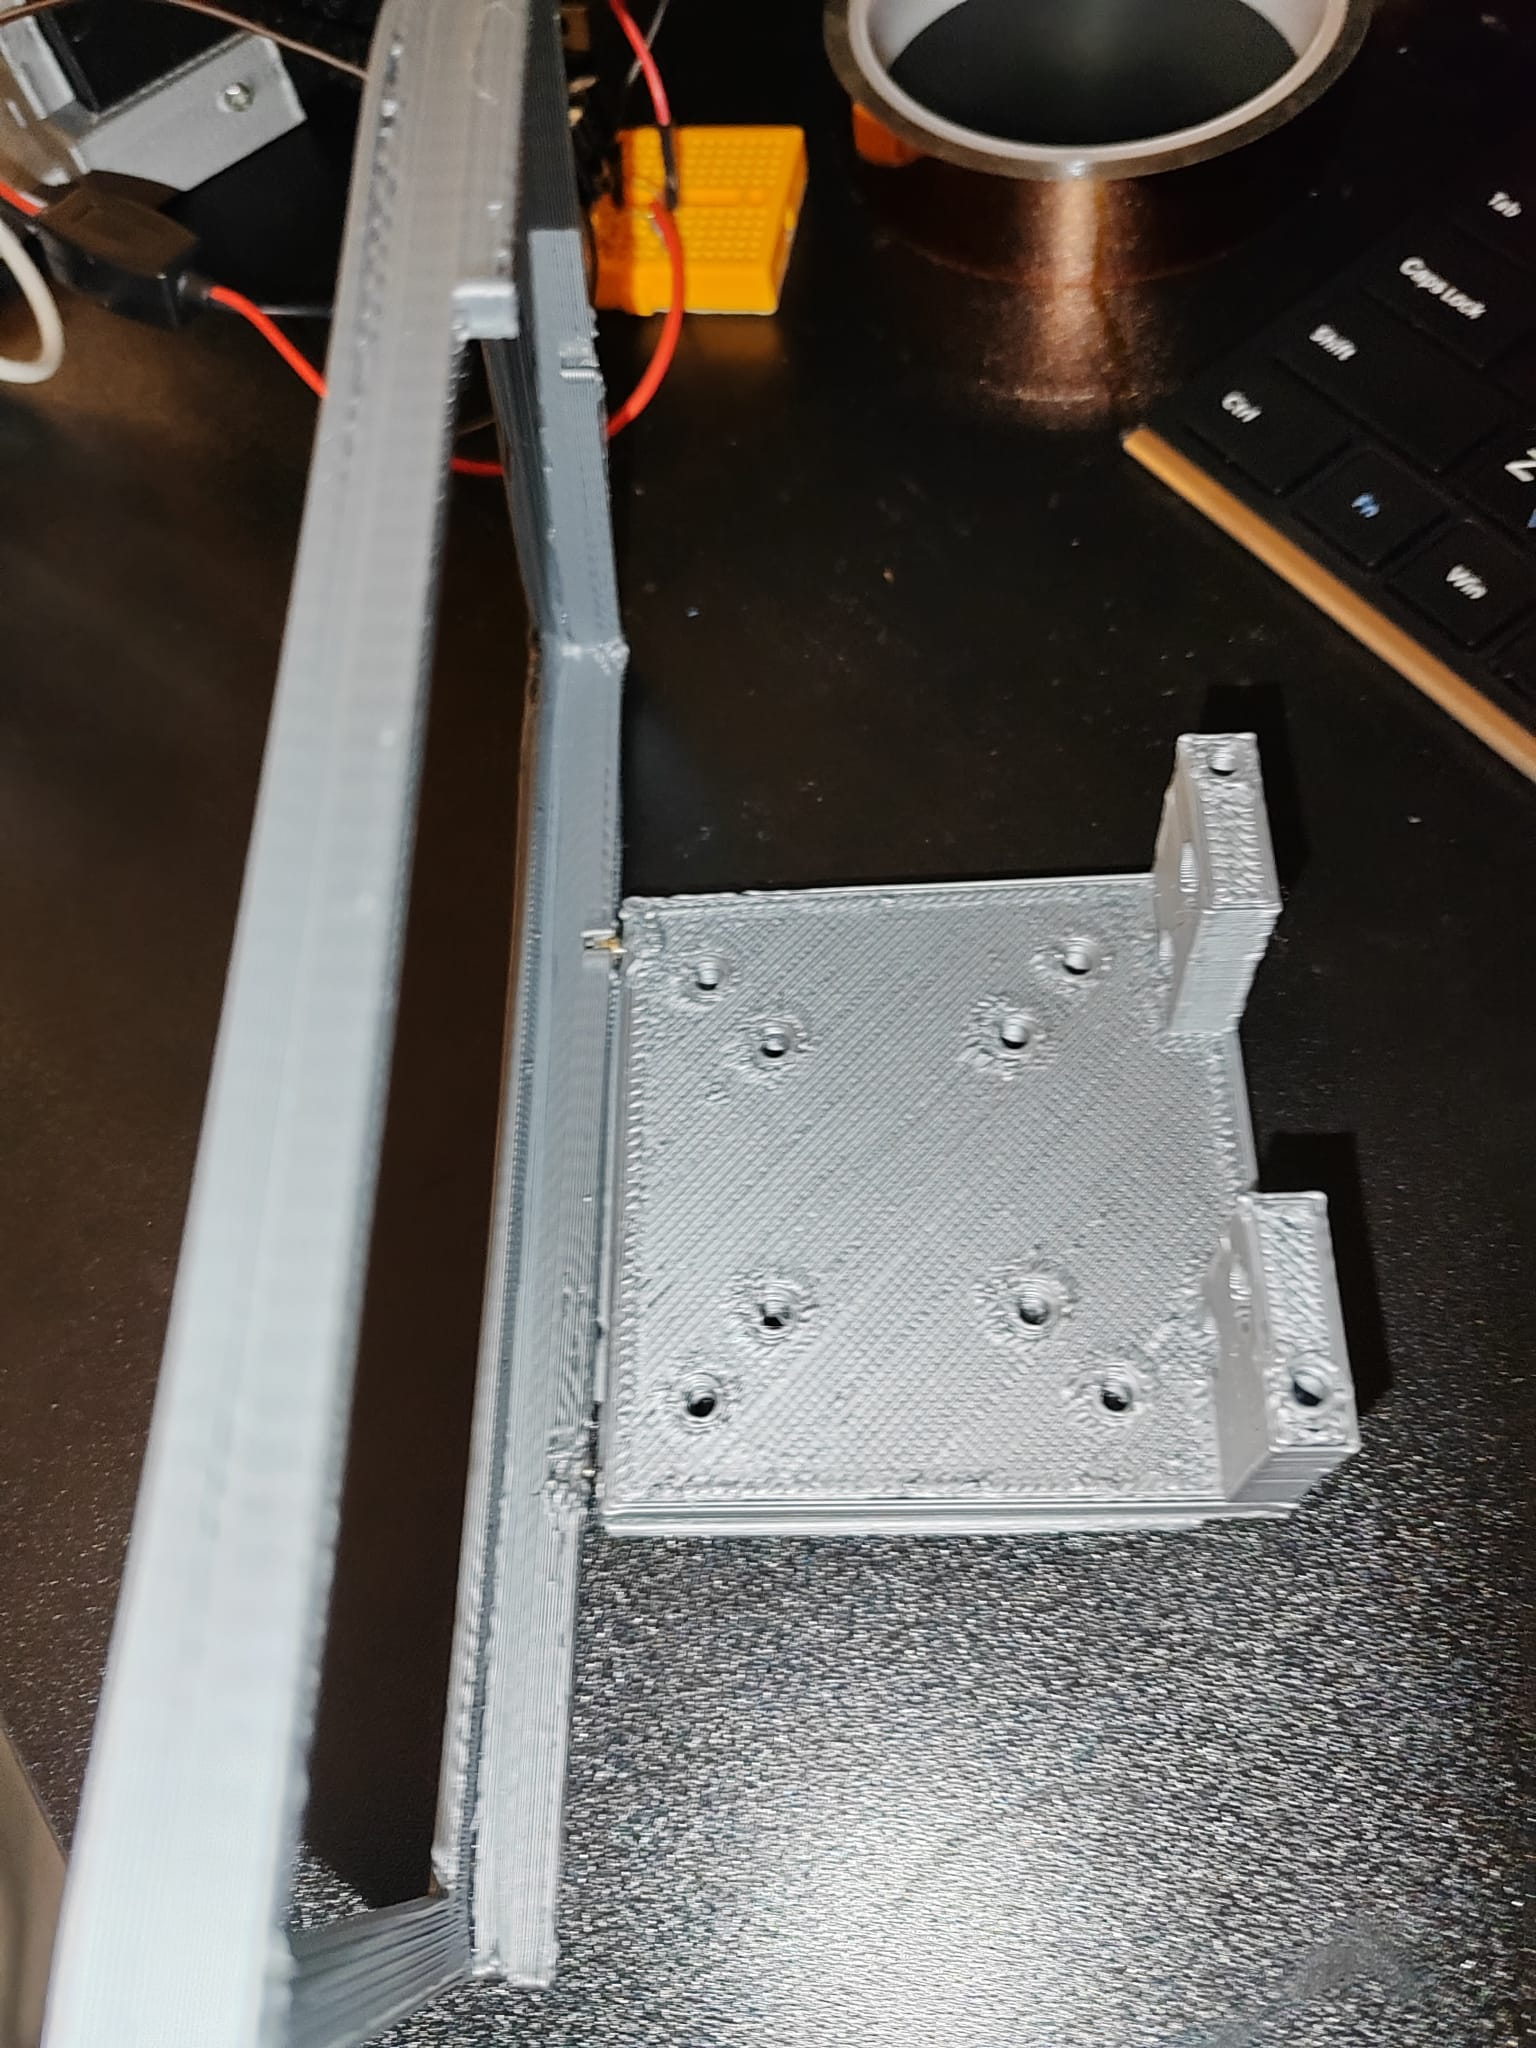
\includegraphics[width=\textwidth,height=5cm, keepaspectratio]{imgs/design/unbracedscreen.jpeg}
    \caption{Unbraced Screen}
    \label{fig:unbracedscreen}
  \end{minipage}
  \hfill
  \begin{minipage}[t]{0.24\textwidth}
    \centering
    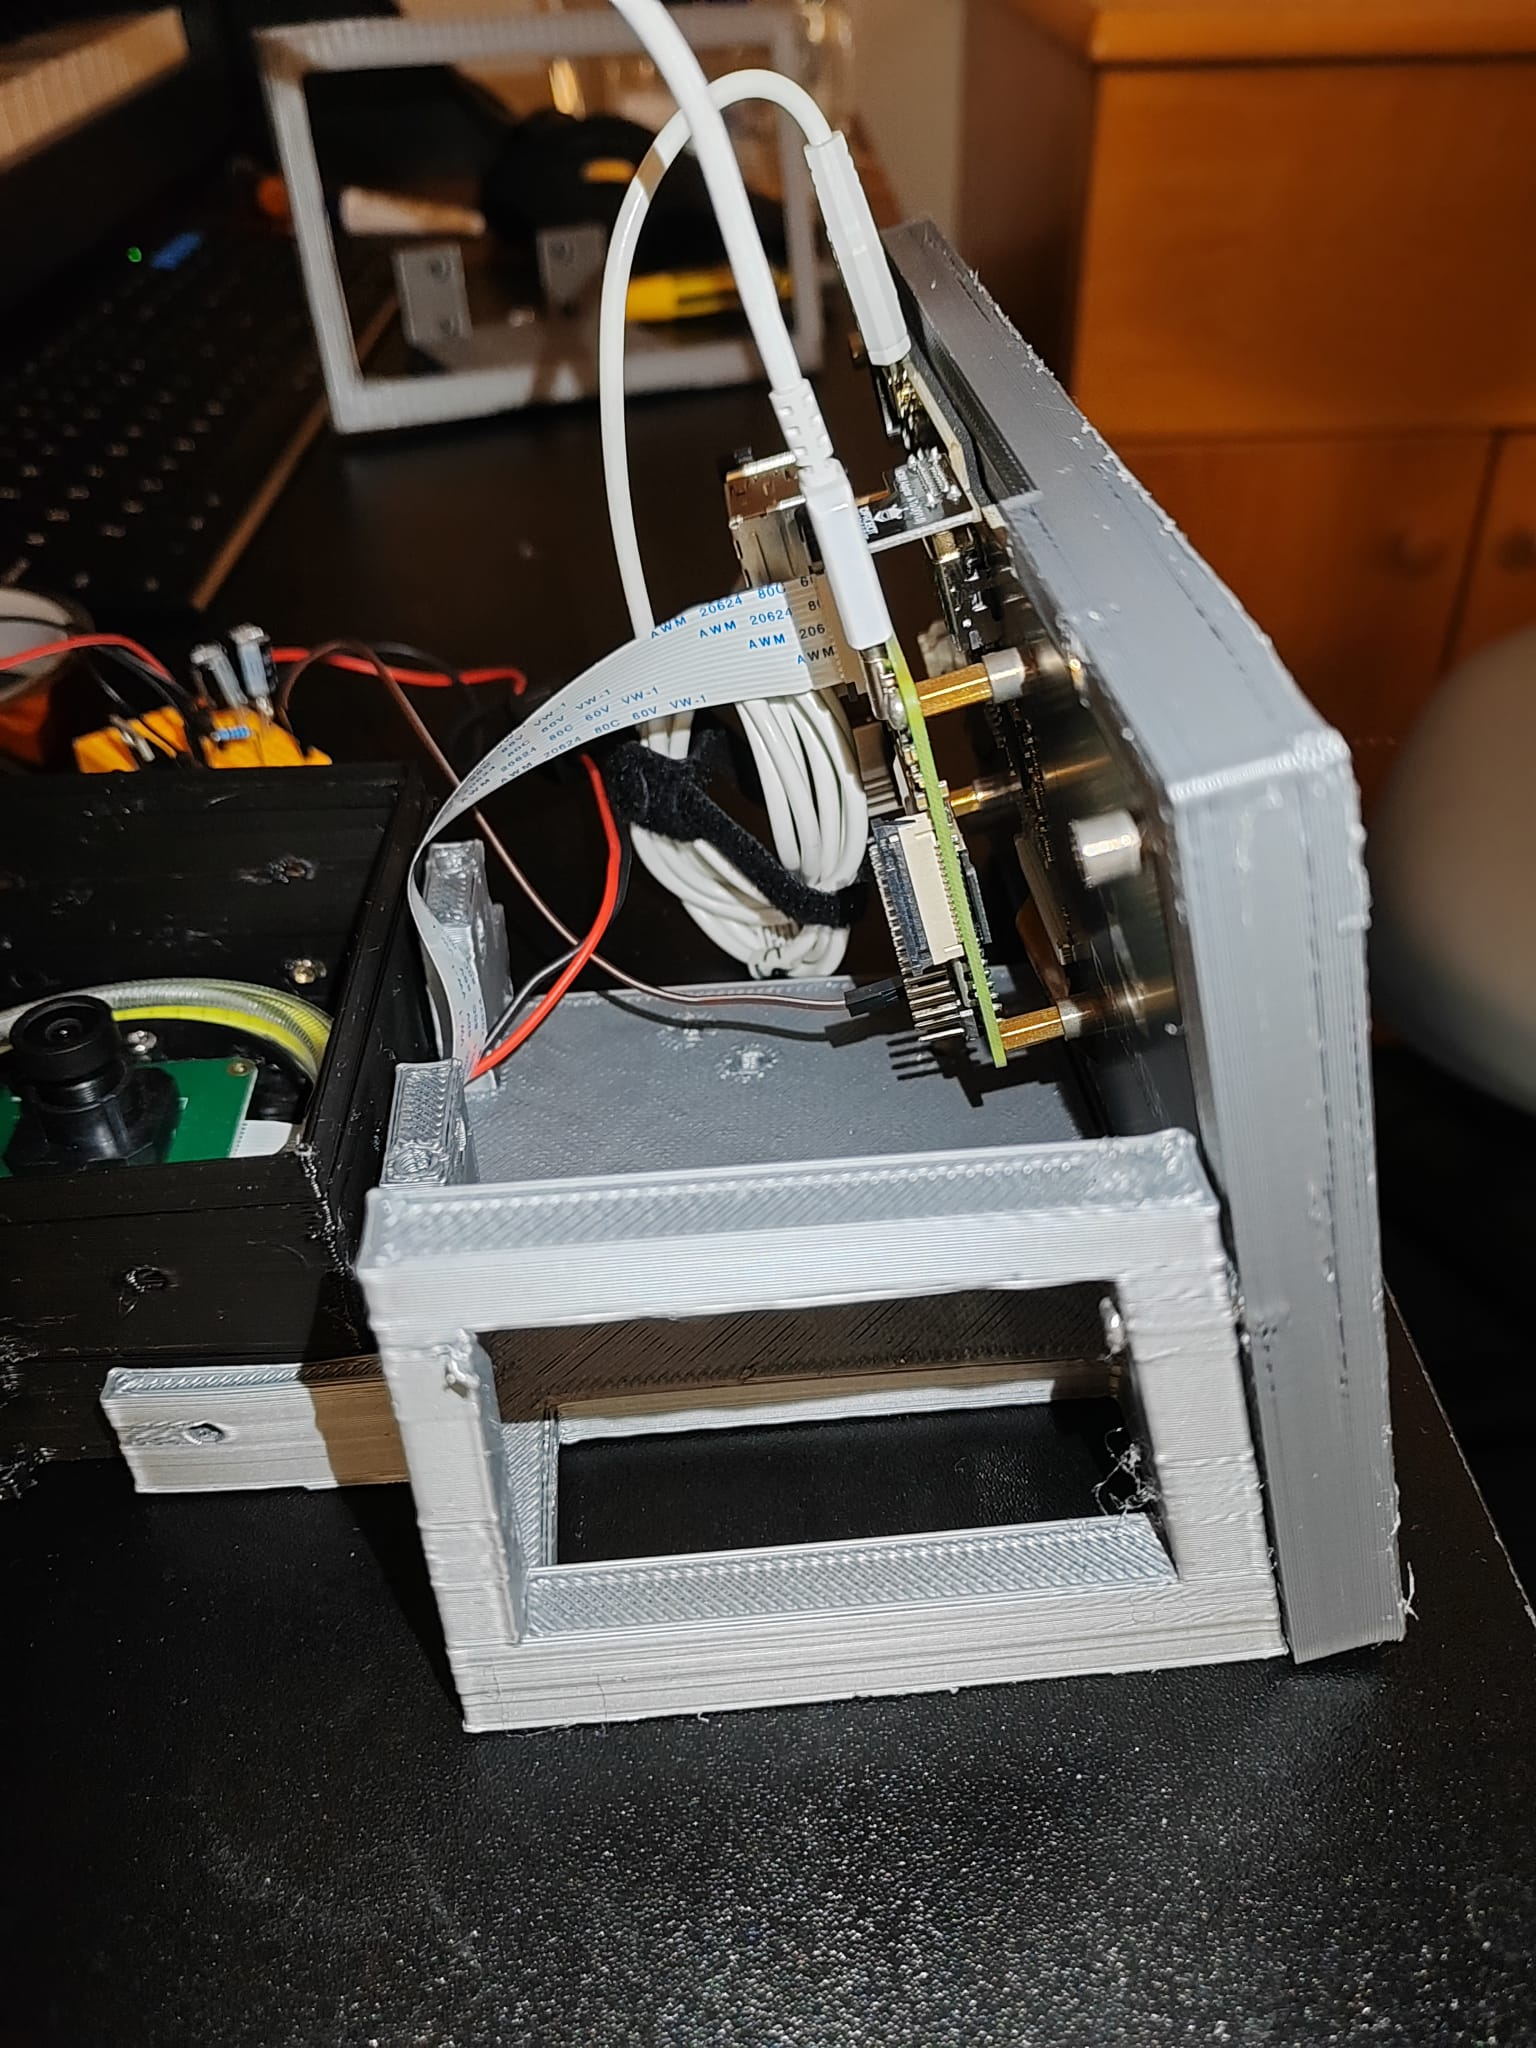
\includegraphics[width=\textwidth,height=5cm, keepaspectratio]{imgs/design/bracedscreen.jpeg}
    \caption{Braced Screen}
    \label{fig:bracedscreen}
  \end{minipage}
  \hfill
  \begin{minipage}[t]{0.24\textwidth}
    \centering
    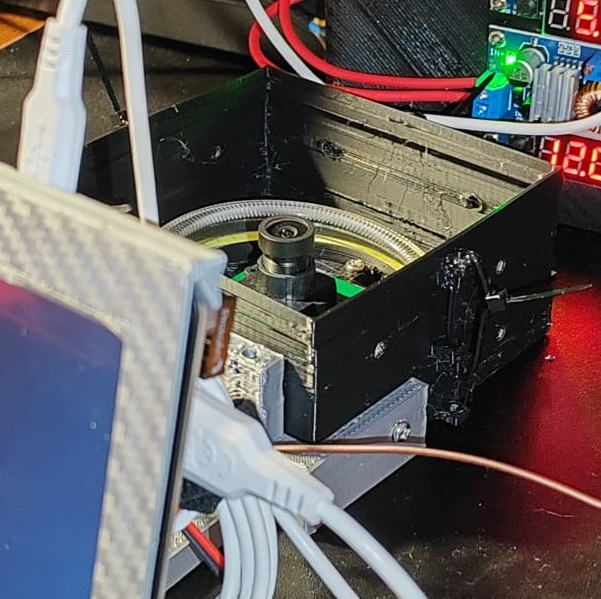
\includegraphics[width=\textwidth,height=5cm, keepaspectratio]{imgs/design/shortcamera.jpeg}
    \caption{Short Camera Housing}
    \label{fig:shortcamera}
  \end{minipage}
  \hfill
  \begin{minipage}[t]{0.24\textwidth}
    \centering
    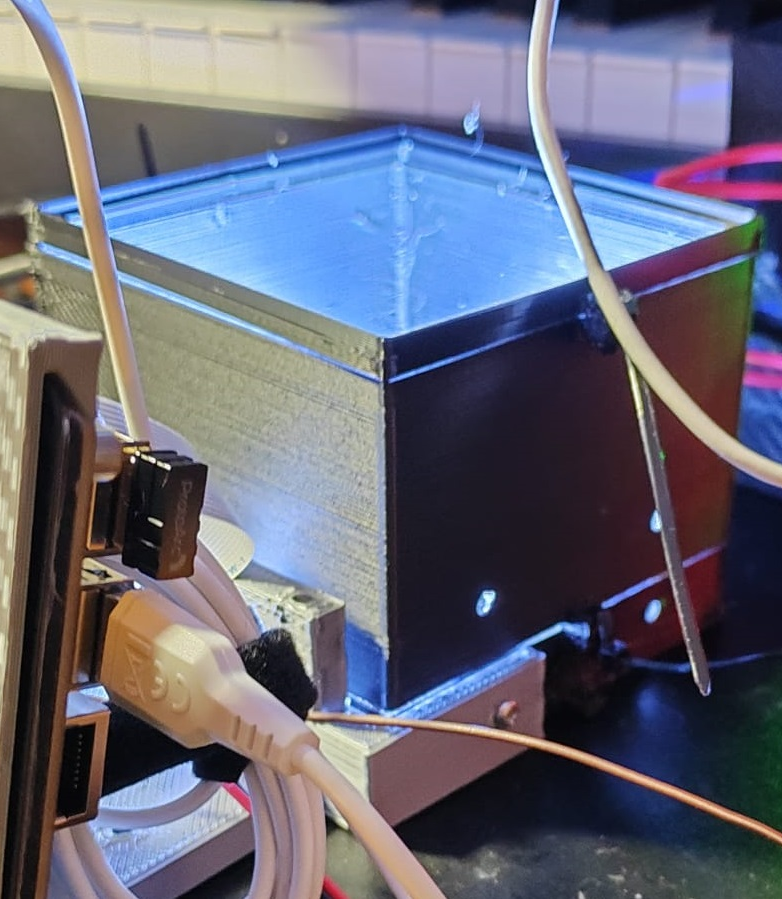
\includegraphics[width=\textwidth,height=5cm, keepaspectratio]{imgs/design/tallcamera.jpeg}
    \caption{Optimal Camera Housing}
    \label{fig:tallcamera}
  \end{minipage}
\end{figure*}
\vspace{-0.5em}
\noindent
However, in the end, none of these could be considered because of the electronics design problem discussed in the following section. \\
\noindent
\textbf{Electronics Design Problems} \\
Attempting to dim the LED Ring resulted in very sporadic flickering, and it did not react with changes to the frequency of the PWM signal despite the MOSFET control circuit shown in Figure \ref{fig:wiringschematic}.
Originally, it was thought that the issue was due to the MOSFET, as initially a MOSFET with a higher gate threshold voltage (IRF520N) was used, and so it was replaced with one with a lower gate threshold voltage.
However, this did not solve the issue, and a capacitor was added in parallel to the LED Ring to buffer the voltage, but to no avail.
The LED Ring seemed to be a simple component with no additional circuitry except for the LEDs, so it was not clear why it was not dimmable. Supervisor Dr. Stott was also unsure as to why it was not dimmable and proposed a different circuit with an inductor and diode but this requires
a much higher switching frequency than the Pi's PWM signal can provide, and so it was not viable. 

For these reasons, and after reviewing the literature as discussed in Section \ref{sec:background}, it was decided that the camera mount was to be redesigned to be down-facing (as a conveyor belt will also be used in the future)
and to replace the LED Ring with a WS2812B LED strip, as these are designed to be dimmable. They are also addressable, however, this is not a feature that is required at this stage of the project.
